\documentclass[conference]{IEEEtran}
\usepackage{graphicx}

\begin{document}

\title{Project Midpoint Report:\\Matrix Profile MPI Implementation}

\author{\IEEEauthorblockN{Richard McNew\IEEEauthorrefmark{1}, Brody Larsen\IEEEauthorrefmark{2}, Feyisa Berisa\IEEEauthorrefmark{3} and Hugh Harps\IEEEauthorrefmark{4}}
\IEEEauthorblockA{Department of Computer Science, Utah State University\\ Logan, Utah, USA\\
\IEEEauthorrefmark{1}a02077329@usu.edu, \IEEEauthorrefmark{2}a01977457@usu.edu, \IEEEauthorrefmark{3}a01676072@usu.edu, \IEEEauthorrefmark{4}a02222128@usu.edu}
}


\maketitle
\begin{abstract}
MPI Implementation of the Matrix Profile
\end{abstract}

\begin{IEEEkeywords}
parallel computation, MPI, data science, Matrix Profile
\end{IEEEkeywords}

\section{Project Thesis}
This project will create an MPI implementation of the Matrix Profile in C++.

\section{Project Details}
Time series data is a collection of observations made sequentially in time.  Time series data is ubiquitous in our modern world and takes the form of sensor data, stock market data, network metrics, application logs, and many other forms.  Analyzing time series data is essential to understanding what is happening and enables informed decision-making and strategic planning.  One recent advancement in time series data analysis is the Matrix Profile \cite{MatrixProfile1}. 

The Matrix Profile is an amazing data structure and set of accompanying algorithms that annotate a time series and make most time series data mining problems easy to solve \cite{MatrixProfile2}. The Matrix Profile is:  1) exact - it allows for time series analysis without false positives or false negatives, 2) parameter-free - unlike many time series data analysis tools, no hyperparameter tuning is needed, 3) space efficient - a matrix profile data structure does not require much space, enabling large datasets to be processed in memory, 4) parallelizable - it is fast to compute on modern hardware, and 5) simple - it is easy to use and fairly easy to understand \cite{Keogh}.   

Most data science work is done in Python.  As a result, most Matrix Profile implementations in use today are written in Python \cite{Stumpy} and rely on the NumPy, SciPy, and Numba Python libraries for vector and matrix data types, numerical and scientific algorithms, and fast just-in-time optimizations.  Creating a Matrix Profile implementation using MPI in C++ will offer organizations that use MPI a way to use the Matrix Profile. 

\section{Tests}
In order to validate the proposed MPI implementation of Matrix Profile in C++ a test suite would need to be created.  The test suite will be created by finding or creating input time series data, running one or more Python Matrix Profile implementations against the input time series data, and capturing the output Matrix Profile data structures.  The MPI Matrix Profile implementation will be validated as correct if the output Matrix Profile data structures match those created by the Python Matrix Profile implementations. 

\section{Anticipated Results}
The MPI-based Matrix Profile implementation will produce the same results as Python-based Matrix Profile implementations and will work in MPI environments.

\section{Project Management System}
Group 010 will use git for version control of all source code, configuration, documentation, and report source documents.  

GitHub is used to host a shared git repository, provide access control, manage pull requests and merges, and provide detailed tracking of issues.

GitHub Issues will be used for sprint planning, story point tracking, backlog tracking, and task assignments. Burndown charts will be generated manually based on GitHub tracking of Issues and Milestones. 

\section{Meeting Plan}
Group 010 will meet each week on Mondays at 8:00 PM on Zoom to end the previous week's sprint, plan for the next sprint, and start the next sprint.  Coordination will also happen by email or phone calls as needed.  Out-of-band meetings may also be held subject to project needs.

\begin{table}
\caption{Groomed List of Tasks Accomplished for Midpoint Report}
\begin{tabular}{|c|c|c|}
\hline
\textbf{Task} & \textbf{Who Worked On It} & \textbf{Story Points} \\ \hline \hline
Share contact info with group members & Brody and Richard & 1 \\ \hline
Decide on meeting plan & Brody and Richard & 2 \\ \hline
Decide on thesis for the project & Brody and Richard & 2 \\ \hline
Create a draft proposal document & Brody and Richard & 2 \\ \hline
Review and revise draft proposal document & Brody, Feyisa, \& Hugh & 3 \\ \hline
Submit completed proposal document & Brody and Richard & 1 \\ \hline
\hline
\end{tabular}
\end{table}

\section{Midpoint Report Burndown Charts}
Burndown charts go here.

%\begin{figure}
%\begin{center}
%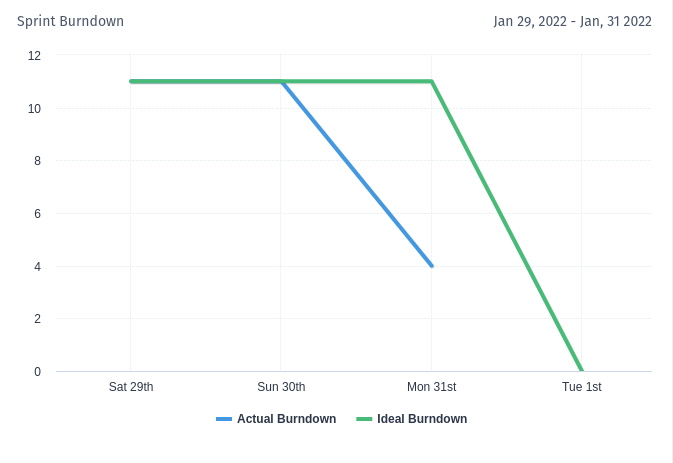
\includegraphics[scale=0.75]{2022-01-29_to_2022-01-31.png}
%\caption{Midpoint Report Burndown Chart}
%\end{center}
%\end{figure}


\bibliographystyle{IEEEtran}

% number is the number of reference labels
\begin{thebibliography}{6}  

\bibitem{MatrixProfile1} Yeh, Chin-Chia Michael, et al. (2016) "Matrix Profile I: All Pairs Similarity Joins for Time Series: A Unifying View that Includes Motifs, Discords, and Shapelets". ICDM:1317-1322.

\bibitem{MatrixProfile2} Zhu, Yan, et al. (2016) "Matrix Profile II: Exploiting a Novel Algorithm and GPUs to Break the One Hundred Million Barrier for Time Series Motifs and Joins". ICDM:739-748.

\bibitem{DynamicTimeWarping} T. Rakthanmanon et al., “Searching and Mining Trillions of Time Series Subsequences under Dynamic Time Warping,” In KDD 2012, 262-270.

\bibitem{Keogh} E. Keogh, \emph{The UCR Matrix Profile Page}, 2021. [Online]. Available: https://www.cs.ucr.edu/~eamonn/MatrixProfile.html.

\bibitem{Stumpy} S.M. Law, (2019). STUMPY: A Powerful and Scalable Python Library for Time Series Data Mining. Journal of Open Source Software, 4(39), 1504.

\bibitem{Pacheco} P. Pacheco. \emph{Parallel Programming with MPI}, Morgan Kaufmann; 1st edition (October 15, 1996), ISBN: 978-1558603394.

\end{thebibliography}

\end{document}
